\section{Introduction}

Consider a set $\cH$ of $n$ \emph{hypotheses}, a set $\cT$ of $m$ \emph{tests} and  an unknown \emph{target hypothesis} $\target\in\cH$ that needs to be discovered through testing.
Each test $t\in\cT$ is a partition of $\cH$, that is, $t$ consists of subsets of $\cH$ such that $x\cap y=\emptyset$ for any $x,y\in t$ and $\bigcup_{x\in t} x=\cH$.
As a result of executing a test $t\in\cT$, \questioner recives a \emph{reply} that reveals $x\in t$ such that $\target\in x$.
That is, the \questioner learns which subset of $\cH$ that belongs to $t$ contains the target.
Each subsequent test is selected by \questioner by taking into acocunt replies from all tests to date.
Without formally stating an optimization criterion we refer to the above as the \emph{Optimal Decision Tree} ($\ProblemDT$) problem.
The goal of \questioner is to output $\target$ while minimizing either the number of tests done in the worst case or on average.
(For formal statemets of our problems see the next section).

We note that the above statement generalizes the classical binary search in (fully or partially) sorted data.
In this work we generalize this proces by considering precedence relation between tests given as an arbitrary partial order $(\cT,\preceq)$.
Then, a test $t$ can be performed only when all its predecesors had to be performed previously (to which we refer as \emph{precedence-closed} solution).
On the applicability side, the binary search itself includes numerous use cases, some of them in the area of biology \cite{BayesianLearnerOptimalNoisyBinarySearch}.
For example, if hypotheses were to represent possible conditions or deseases, and each test distinguishes between some pairs of hypotheses, then precedence constaints would represent some ordering on performing tests.
These may be enforced e.g. by cost measures (like executing several `cheaper' tests whose outcome may eliminate the need of executing a more expensive one), or by an expert.

The method to address the optimal decision tree problems is through a series of `reductions' between other optimization problems.
By this we mean an approach, where a particular algorithm for one problem implies existence of an algorithm for the other.
Particularly, we study a set cover problem with precedences:
We are given a set $\cU$ of $n$ items, a collection $\cS$ of $m$ subsets of $\cU$, such that $\bigcup_{S\in\cS}S=\cU$, an arbitrary partial order $(\cS,\preceq)$ on these subsets and an integer $k$.
We say that a subfamily $\cC\subseteq\cS$ \emph{covers} at least $k$ items from $\cU$ if $\spr{\bigcup_{C\in\cC}C}\geq k$.
We ask for a $\cC\subseteq\cS$ that covers at least $k$ items from $\cU$ and is \emph{precedence-closed}, that is, for each $x\in\cC$ and each $y\in\cS$ such that $y\preceq x$ it holds $y\in\cC$.
The approximation algorithms that we propose en route, e.g. for precedence constrained set cover, are of independent interest.

% \medskip
% \paraTitle{Outline.}
% In the next section we formally state all problems we address in this work.
% Section~\ref{sec:our-results} gives an overview of the main results of this work.
% Section~\ref{sec:AL} provides approximation algorithm for the above decision tree problem, assuming there exist certain approximations for variants of set cover.
% The latter are developed in Section~\ref{sec:SC}.
% Finally, set cover is solved via dense subfamily approximation from Section~\ref{sec:MDPCS}.
% The algorithms are supplemented with a number of inapproximability results in Section~\ref{sec:hardness}.

% Consider following problems:
% \begin{itemize}
%   \item  The \emph{Precedence Constrained Bayesian Decision Tree Problem} consists a set of $\mathcal{H}$ of $n$ hypothesis, a set $\cT$ of $m$ tests and a DAG (directed acyclic graph) $\mathcal{F} = \brc{\cT, \preceq}$ encoding the precedence constraints between available tests. Among $\mathcal{H}$ a hidden hypothesis is required to be encovered. To do so, the learner is allowed to perform tests, each of which reveals partial information about the hidden hypothesis. Upon receiving this information, the learner actively selects the next test to be performed. Importantly, in order to perform such test the learner needs to perform all of its predecesors in $\mathcal{F}$ first. The goal is to uncover the hidden hypothesis while performing as few tests as possible. Depending on the chosen criterion we distinguish between the \emph{Precedence Constrained Worst Case Decision Tree} (PCWCDT) and \emph{Precedence Constrained Average Case Decision Tree} (PCACDT) problems.
%   \item The \emph{Precedence Constrained Covering Problem} consists of a set of $n$ items $\mathcal{U}$, a collection $\mathcal{S}$ of $m$ subsets of $\mathcal{U}$ that cover these items, and a DAG $\mathcal{F} = \brc{\mathcal{S}, \preceq}$ encoding the precedence constraints between available subsets. The goal is to select a sequence of tests that covers at least $K$ items. Depending on the chosen criterion we distinguish between the \emph{Precedence Constrained Set Cover} (PCSC) and \emph{Precedence Constrained Min-Sum Set Cover} (PCMSSC) problems. In the first we are only interested in minimizing the number of selected subsets, while in the second we want to minimize the average time it takes to cover an item.
% \end{itemize}

\subsection{Problem formulations and outline} \label{sec:problems}

\DD{ta sekcja jest w miare ulozona pod ustalenia na discord; z wyjatkiem dwoch ostatnich problemow -- do decyzji czy potrzebne}

After introducing necessary notation in Section~\ref{sec:preliminaries}, we provide algorithms (cf. Section~\ref{sec:AL}) for the decision tree problems.
\begin{problem}[Precedence Constrained Worst Case Decision Tree ($\ProblemPCWCDT$)] \label{problem:PCWCDT}
Given a set of hypotheses $\cH$, a set of tests $\cT$ and a precedence relation $(\cT,\preceq)$ on tests, find a precedence-closed decision tree strategy that outputs the target hypothesis by performing the minimum number of tests in the worst case.
\end{problem}
\begin{problem}[Precedence Constrained Average Case Decision Tree ($\ProblemPCACDT$)] \label{problem:PCACDT}
Given a set of hypotheses $\cH$, a set of tests $\cT$ and a precedence relation $(\cT,\preceq)$ on tests, find a precedence-closed decision tree strategy that outputs the target hypothesis $\target$ and minimizes the sum $\sum_{h\in\cH}c(h)$, where $c(h)$ is the number of tests performed when $h=\target$.
\end{problem}
Whenever the criterion is not important or we want to make a claim that applies both to $\ProblemPCWCDT$ and $\ProblemPCACDT$, we use the symbol $\ProblemPCDT$ to refer to a \emph{Precedence Constrained Decision Tree} instance.

The algorithms for the above are conditioned on existence of approximations for the set cover.
These in turn are obtained via a reduction from a problem of finding a maximum density subset (cf. Section~\ref{sec:MDPCS}).
The \emph{density} $\Delta$ of a nonempty subfamily $\cA$ on a universum $X$ ($A\subseteq X$ for each $A\in\cA$) is
\[
\Delta\br{\cA, X} \equiv \frac{\spr{\cov\br{\cA, X}}}{\spr{\cA}}
\]
For convenience, we define $\Delta\br{\emptyset, X} < 0$.
We also write $\Delta\br{\cA}$ when $X$ is the universum.
\begin{problem}[Max-Density Precedence-Closed Subfamily ($\ProblemMDPCS$)]
Given a universum $\cU$ of $n$ items, a family $\cG$ of $m$ subsets of $\cU$ and a precedence relation $(\cG,\preceq)$, find a precedence-closed subfamily $\cA \subseteq \mathcal{G}$ that maximizes $\Delta\br{\cA}$.
\end{problem}
We will also need a `bounded' version:
\begin{problem}[Bounded Max-Density Precedence-Closed Subfamily ($\ProblemBMDPCS$)]
Given a universum $\cU$ of $n$ items, a family $\cG$ of $m$ subsets of $\cU$, a precedence relation $(\cG,\preceq)$ and an integer $B>0$, find a precedence-closed subfamily $\cA \subseteq \mathcal{G}$ that maximizes $\Delta\br{\cA}$ and $\spr{\cA}\leq B$.
\end{problem}

Having proved the necessary claims on $\ProblemMDPCS$ and $\ProblemBMDPCS$, we develop in Section~\ref{sec:SC} the algorithms for set cover variants introduced below.
For any partial order $(X,\preceq)$ and $S\subseteq X$ let $\closure{S}$ denote the minimal precedence-closed subset of $X$.
For a family of sets $\cA$ its \emph{coverage} is $\cov\br{\cA}=\bigcup_{A\in\cA}A$, and by extension, $\cov\br{\cA, X} = \cov\br{\cA} \cap X$ for any set $X$.
\begin{problem}[Precedence Constrained Set Cover ($\ProblemPCSC$)]
Given a universum $\cU$ of $n$ items, a family $\cS$ of $m$ subsets of $\cU$, a precedence relation $(\cS,\preceq)$ and $0<f<1$, find a precedence-closed subfamily $\cC\subseteq\cS$ that covers at least $fn$ items and minimizes $\spr{\cC}$.
\end{problem}
A permutation $\br{C_1,\ldots,C_l}$ of the elements in $\cC$ is \emph{consistent} with the partial order $(\cS,\preceq)$ if for any $C_i$ and $C_j$ such that $C_i\preceq C_j$ it holds $i<j$.
The \emph{coverage time} of a $x\in\cov\br{\cC}$ is the minimum index $i$ such that $x\in C_i$.
\begin{problem}[Precedence Constrained Min-Sum Set Cover ($\ProblemPCMSSC$)]
Given a universum $\cU$ of $n$ items, a family $\cS$ of $m$ subsets of $\cU$, a precedence relation $(\cS,\preceq)$ and $0<f<1$, find a precedence-closed sequence $(C_1,\ldots,C_l)$ that covers at least $fn$ items and minimizes the sum of coverage times of the elements in $C_1\cup\cdots\cup C_l$.
\end{problem}
\begin{problem}[Budgeted Precedence Constrained Set Cover ($\ProblemBPCSC$)]
Given a universum $\cU$ of items, a family $\cS$ of subsets of $\cU$ and a budget $B>0$, find a precedence-closed set cover $\cC$ that maximises the number of covered items and satisfies $\spr{\cC}\leq B$.
\end{problem}

Our results are supplemented with a number of inapproximability results in Section~\ref{sec:hardness}.


\DD{A te dwa problemy to na razie resztowka, ktora gdzies powinna trafic}
\begin{problem}[Group Steiner Tree (GST)]
Given an undirected graph $G = (V, E)$ with edge costs, a root vertex $r \in V$, and groups $g_1, \ldots, g_k \subseteq V$, find a minimum-cost tree $T$ rooted at $r$ that contains at least one vertex from each group $g_i$.
\end{problem}

\begin{conjecture}[Planted Dense Subgraph (PDS) Conjecture]
For any constants $\beta < \alpha$ and any $k\geq \sqrt{N}$, there is no polynomial time algorithm that can distinguish between the following two distributions of graphs with any advantage $\epsilon > 0$: (1) With probability 1/2, an Erdős-Renyi graph $G(N, N^{\alpha - 1})$, (2) With probability 1/2, an Erdős-Renyi graph $G(N, N^{\alpha - 1})$ with a planted subgraph of size $k$ and edge density $k^{\beta - 1}$.
\end{conjecture}

\begin{problem}[Precedence constrained test cover (PCTC)]
Given a set $\cH$ of $n$ hypotheses, a set $\cT$ of $m$ tests, and a partial order $\brc{\cT, \preceq}$ encoding precedence constraints for $\cT$, find a precedence-closed subfamily of tests that distinguishes all pairs of hypotheses.
\end{problem}


\subsection{Related Work}

\paragraph{Optimal Decision Tree}
Optimal decision tree is among the classical problems in computer science and has been studied extensively, starting with Garey \cite{GareyPerfBoundsOnSplittingAlgForBinTesting} in the 1970s. 
Since that time, it has gathered a lot of attention due to its numerous applications which include medical diagnosis, troubleshooting, active learning, and information retrieval. 
This problem is usually studied under two different optimization criteria: minimizing the worst-case cost and minimizing the average-case cost. 
Both versions of the problem are known to be NP-hard and cannot be approximated within an $o\br{\log n}$ factor \cite{ConstructOptimalBinaryDecisionTreesIsNPComplete,HardnessOfMinHeightDTP,ApproximatingDecisionTreesMultiwayBranches,DiagnosisDetermination}. Moreover, this bound is known to be tight and several $\cO(\log n)$-approximation algorithms for both non-uniform probabilities and cost average-case \cite{OptimalSplitTreeProblem,AnalysisGreedyActiveLearning,ApproximatingDecisionTreesMultiwayBranches,AverageCaseActiveLearningWithCosts,ApproximatingOptimalBinaryDecisionTrees,DTsforEntIdent,ApproxAlgsForOptDTsAndAdapTSPProblems,DiagnosisDetermination,AdaptiveSubmodularRankingAndRouting,AdaptivityInAdaptiveSubmodularity,MinimumCostAdaptiveSubmodularCover} as well as worst case \cite{DecisionTreesForGeometricModels,TheCostComplexityOfInteractiveLearning,DiagnosisDetermination}. Despite the hardness of the problem several special cases are known to have $o\br{\log n}$-approximation algorithms. For average case, this includes when tests have a constant number of possible outcomes and all probabilities and costs are uniform an $\cO\br{\log n/\log \log n}$-approximation is known \cite{TightAnalysisGreedyUniformDecisionTree}. This variant cannot be approximated within $\br{4-\epsilon}$ factor for any $\epsilon > 0$ unless P = NP \cite{DTsforEntIdent}. Moreover achieving any approximation factor above $9$ is not NP-hard assuming ETH \cite{TightAnalysisGreedyUniformDecisionTree}.
For worst case, when the underlying search space is a partially ordered set with a maximum element and costs are uniform an $\cO\br{\log n/\log \log n}$-approximation is known \cite{EdgeRankingSearchingPartialOrders}.


\paragraph{Searching in Trees}
For a special case when the instance represents searching in a tree, i.e., the set of hypothesis represents vertices of a tree and tests inform about the direction of the target placement with respect to the queried element (depending on the model, either vertices or edges can be queried), the problem has also been extensively studied. For uniform costs and worst-case criterion, a linear time exact algorithm is known for both edge query and vertex query variant \cite{Schaffer1989OptNodeRankOfTsInLinTime,OnakParys2006GenOfBSSInTsAndFLikePosets,Mozes_Onak2008FindOptTSStartInLinTime}. For average case, uniform costs and vertex queries an FPTAS is known \cite{SearchTreesOnGraphs}. For edge queries the problem is known to be NP-hard \cite{OnTheComplexityOfSearchingInTreesAverageCaseMinimization} and a greedy strategy achieves $3/2$-approximation \cite{TightApproximationBoundsOnASimpleAlgorithmForMinimumAverageSearchTimeInTrees}. For the case of non-uniform costs, the vertex query model generalizes edge query model. For worst case, the problem is known to be NP-hard \cite{EdgeRankingOfWeightedTrees,TheBinaryIdentificationProblemForWeightedTrees,OnTheTreeSearchProblemWithNonUniformCosts} and the best known approximation ratio is $\br{\sqrt{\log n}}$ \cite{ApproximationStrategiesforGeneralizedBinarySearchinWeightedTrees}.
The average case is also known to be NP-hard and an $\br{4+\epsilon}$-approximation FPTAS is known \cite{szyfelbein2025approximatingaveragecasegraphsearch}.

\paragraph{Set Cover with precedence constraints}

Set cover is the most important problem in combinatorial approximation algorithms.
It is well known that the greedy algorithm achieves an $H_n$-approximation for set cover \cite{GreedyHeuristicSetCoverProblem}, where $H_n=\cO\br{\log n}$ is the $n$-th harmonic number. Converesely, this is tight as set cover cannot be approximated within a $(1-\epsilon)\ln n$ factor for any $\epsilon > 0$ unless P=NP \cite{AnalyticalApproachToParallelRepetition}. The Min-Sum Set Cover is a version of the problem in which the goal is to minimize the average cover time of element. For this version, the greedy algorithm achieves $4$-approximation algorithm \cite{ApproximatingMinSumSetCover}, which is tight. When allowing arbitrary precedence constraints the problem admits an $\cO\br{\sqrt{m}}$-approximation algorithm and cannot be approximated within a $\cO\br{m^{1/6-\epsilon}}$ factor \cite{PCMSSC} subject to the Planted Dense Subgraph Conjecture \cite{OnApproxTargetSetSelection}.

\subsection{Our results and techniques} \label{sec:our-results}
\DD{ta sekcja jest under construction; do mocniejszego przerobienia}

Our first theorem is due to Theorem~\ref{thm:alphaPCWCDT}.
\begin{theorem} \label{thm:generalPCWCDT}
There exists a polynomial-time $\bigo(\sqrt{m}\log n)$-approximation algorithm for the $\ProblemPCWCDT$, where $n$ is the number of hypotheses and $m$ is the number of tests.
\end{theorem}
Theorem~\ref{thm:alphaPCWCDT} relies on a bicriteria optimization algorithm for $\ProblemPCSC$ stated in Theorem~\ref{thm:MDPCStoPCSC} which in turn is obtained via an approximation algorithm for a problem called \emph{Max-Density Precedence-Closed Subfamily} ($\ProblemMDPCS$) given in \cite{PCMSSC}.
\DD{(byc moze definicja MDPCS)}
As a corollary of Theorem~\ref{thm:MDPCStoPCSC}, we obtain the following result regarding $\ProblemPCSC$.
\begin{theorem} \label{thm:generalPCSC}
There exists a polynomial-time $\bigo(\sqrt{m}f)$-approximation algorithm for $\ProblemPCSC$, where $m$ is the number of subsets over the universum of size $n$ and $f=k/n$, where $k$ is the required number of elements to be covered.
\end{theorem}


\begin{theorem} \label{thm:generalPCACDT}
There exists a polynomial-time $\bigo(\sqrt{m}\log n)$-approximation algorithm for $\ProblemPCACDT$, where $m$ is the number of sets over the universum of size $n$.
\end{theorem}

\begin{theorem} \label{thm:generalPCMSSC}
There exists a polynomial-time $\bigo(\sqrt{m})$-approximation algorithm for $\ProblemPCMSSC$, where $m$ is the number of sets over the universum.
\end{theorem}



% \DD{Ten przykład jest super, ale chyba musimy znaleźć sposób na jego kompresję, tzn. nie stać nas na zapłacenie całej strony; około 1/3 strony byłaby ok (może tabelka obok drzewa decyzyjnego (moze zamiana kolumn vs wierszy aby ją powęzić, a może mocno zminimalizować przestrzeń między kolumnami, a partial order jako łuki pomiędzy etykietami wierszy tabelki?); też do przemyślenia gdzie ten przykład umieścić (raczej nie w ``contribution'', ale albo w intro, albo w preliminaries chyba}
% \begin{figure}[htb!]
% \centering
% \centering

\begin{minipage}[t]{\textwidth}
\centering
\scalebox{0.76}{
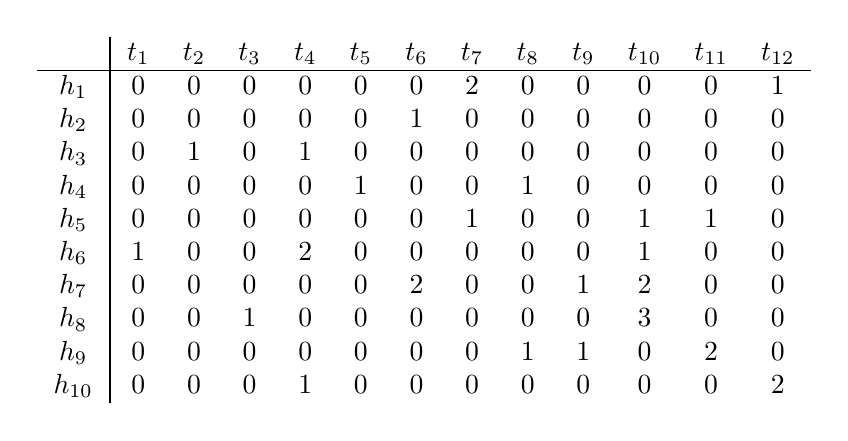
\begin{tikzpicture}[
    node distance=1cm,
    test/.style={circle, draw, thick, minimum size=0.6cm},
    decision/.style={circle, draw, thick, minimum size=0.55cm},
    leaf/.style={circle, draw, thick, fill=green!20, minimum size=0.5cm},
    arrow/.style={->, thick}
]

% Table of hypotheses vs tests (10 hypotheses, 12 tests, unbalanced outcomes)
\node[] at (0,0) {
\begin{tabular}{c|cccccccccccc}
 & $t_1$ & $t_2$ & $t_3$ & $t_4$ & $t_5$ & $t_6$ & $t_7$ & $t_8$ & $t_9$ & $t_{10}$ & $t_{11}$ & $t_{12}$ \\
\hline
$h_1$ & 0 & 0 & 0 & 0 & 0 & 0 & 2 & 0 & 0 & 0 & 0 & 1 \\
$h_2$ & 0 & 0 & 0 & 0 & 0 & 1 & 0 & 0 & 0 & 0 & 0 & 0 \\
$h_3$ & 0 & 1 & 0 & 1 & 0 & 0 & 0 & 0 & 0 & 0 & 0 & 0 \\
$h_4$ & 0 & 0 & 0 & 0 & 1 & 0 & 0 & 1 & 0 & 0 & 0 & 0 \\
$h_5$ & 0 & 0 & 0 & 0 & 0 & 0 & 1 & 0 & 0 & 1 & 1 & 0 \\
$h_6$ & 1 & 0 & 0 & 2 & 0 & 0 & 0 & 0 & 0 & 1 & 0 & 0 \\
$h_7$ & 0 & 0 & 0 & 0 & 0 & 2 & 0 & 0 & 1 & 2 & 0 & 0 \\
$h_8$ & 0 & 0 & 1 & 0 & 0 & 0 & 0 & 0 & 0 & 3 & 0 & 0 \\
$h_9$ & 0 & 0 & 0 & 0 & 0 & 0 & 0 & 1 & 1 & 0 & 2 & 0 \\
$h_{10}$ & 0 & 0 & 0 & 1 & 0 & 0 & 0 & 0 & 0 & 0 & 0 & 2 \\
\end{tabular}
};

\end{tikzpicture}
}
\normalsize
\caption*{(a) Hypotheses and tests table}
\end{minipage}

\begin{minipage}[t]{0.43\textwidth}
\centering
\scalebox{0.78}{
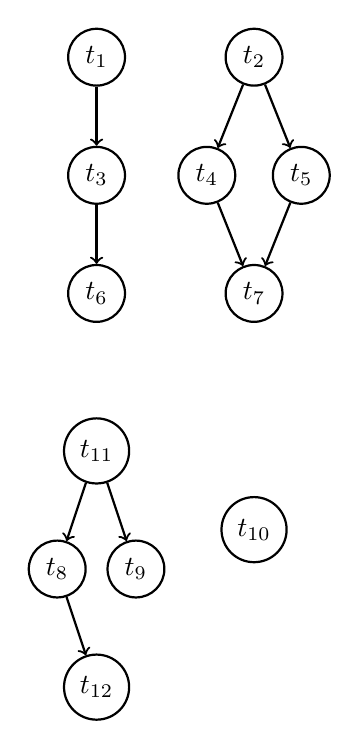
\begin{tikzpicture}[
    node distance=1cm,
    test/.style={circle, draw, thick, minimum size=0.6cm},
    arrow/.style={->, thick}
]

% DAG with 4 components (2 components on top, 2 below)
% Component 1 (top left)
\node[test] (t1) at (0.5,0) {$t_1$};
\node[test] (t3) at (0.5,-1.5) {$t_3$};
\node[test] (t6) at (0.5,-3) {$t_6$};
\draw[arrow] (t1) -- (t3);
\draw[arrow] (t3) -- (t6);

% Component 2 (top right)
\node[test] (t2) at (2.5,0) {$t_2$};
\node[test] (t4) at (1.9,-1.5) {$t_4$};
\node[test] (t5) at (3.1,-1.5) {$t_5$};
\node[test] (t7) at (2.5,-3) {$t_7$};
\draw[arrow] (t2) -- (t4);
\draw[arrow] (t2) -- (t5);
\draw[arrow] (t4) -- (t7);
\draw[arrow] (t5) -- (t7);

% Component 3 (bottom left)
\node[test] (t11) at (0.5,-5) {$t_{11}$};
\node[test] (t8) at (0,-6.5) {$t_8$};
\node[test] (t9) at (1,-6.5) {$t_9$};
\node[test] (t12) at (0.5,-8) {$t_{12}$};
\draw[arrow] (t11) -- (t8);
\draw[arrow] (t11) -- (t9);
\draw[arrow] (t8) -- (t12);

% Component 4 (isolated node, bottom right)
\node[test] (t10) at (2.5,-6) {$t_{10}$};

\end{tikzpicture}
}
\normalsize
\caption*{(b) Precedence}
\end{minipage}
\hfill
\begin{minipage}[t]{0.55\textwidth}
\centering
\scalebox{0.78}{
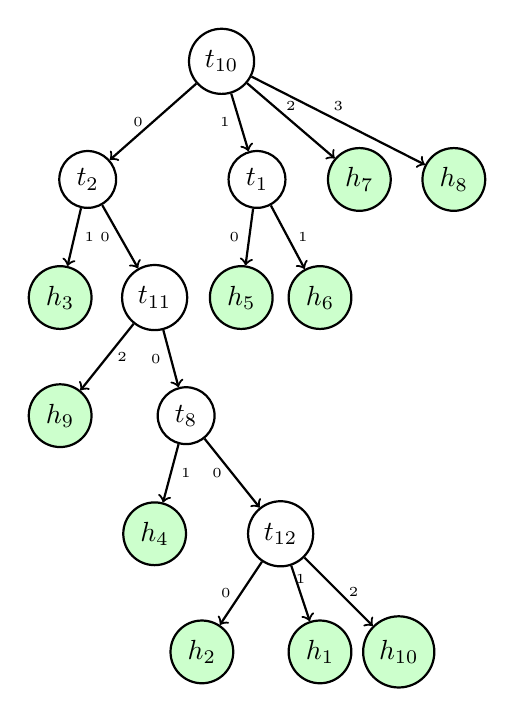
\begin{tikzpicture}[
    node distance=1cm,
    decision/.style={circle, draw, thick, minimum size=0.55cm},
    leaf/.style={circle, draw, thick, fill=green!20, minimum size=0.5cm},
    arrow/.style={->, thick}
]

% Decision tree built from table analysis
% Root: t10 (separates: h5→1, h6→1, h7→2, h8→3, rest→0)
\node[decision] (root) at (4.25,0) {$t_{10}$};

% t10=0: {h1,h2,h3,h4,h9,h10}
\node[decision] (n1) at (2.55,-1.5) {$t_2$};
% t10=1: {h5,h6}
\node[decision] (n2) at (4.7,-1.5) {$t_1$};
% t10=2: {h7}
\node[leaf] (h7) at (6,-1.5) {$h_7$};
% t10=3: {h8}
\node[leaf] (h8) at (7.2,-1.5) {$h_8$};

% t10=0, t2=0: {h1,h2,h4,h9,h10}
\node[decision] (n3) at (3.4,-3) {$t_{11}$};
% t10=0, t2=1: {h3}
\node[leaf] (h3) at (2.2,-3) {$h_3$};

% t10=1, t1=0: {h5}
\node[leaf] (h5) at (4.5,-3) {$h_5$};
% t10=1, t1=1: {h6}
\node[leaf] (h6) at (5.5,-3) {$h_6$};

% t10=0, t2=0, t11=0: {h1,h2,h4,h10}
\node[decision] (n4) at (3.8,-4.5) {$t_8$};
% t10=0, t2=0, t11=1: {h5} - but h5 already separated
% t10=0, t2=0, t11=2: {h9}
\node[leaf] (h9) at (2.2,-4.5) {$h_9$};

% t10=0, t2=0, t11=0, t8=0: {h1,h2,h10}
\node[decision] (n5) at (5,-6) {$t_{12}$};
% t10=0, t2=0, t11=0, t8=1: {h4}
\node[leaf] (h4) at (3.4,-6) {$h_4$};

% t10=0, t2=0, t11=0, t8=0, t12=0: {h2}
\node[leaf] (h2) at (4,-7.5) {$h_2$};
% t10=0, t2=0, t11=0, t8=0, t12=1: {h1}
\node[leaf] (h1) at (5.5,-7.5) {$h_1$};
% t10=0, t2=0, t11=0, t8=0, t12=2: {h10}
\node[leaf] (h10) at (6.5,-7.5) {$h_{10}$};

% Edges
\draw[arrow] (root) -- (n1) node[midway, left, font=\tiny] {0};
\draw[arrow] (root) -- (n2) node[midway, left, font=\tiny] {1};
\draw[arrow] (root) -- (h7) node[midway, above, font=\tiny] {2};
\draw[arrow] (root) -- (h8) node[midway, above, font=\tiny] {3};

\draw[arrow] (n1) -- (n3) node[midway, left, font=\tiny] {0};
\draw[arrow] (n1) -- (h3) node[midway, right, font=\tiny] {1};

\draw[arrow] (n2) -- (h5) node[midway, left, font=\tiny] {0};
\draw[arrow] (n2) -- (h6) node[midway, right, font=\tiny] {1};

\draw[arrow] (n3) -- (n4) node[midway, left, font=\tiny] {0};
\draw[arrow] (n3) -- (h9) node[midway, right, font=\tiny] {2};

\draw[arrow] (n4) -- (n5) node[midway, left, font=\tiny] {0};
\draw[arrow] (n4) -- (h4) node[midway, right, font=\tiny] {1};

\draw[arrow] (n5) -- (h2) node[midway, left, font=\tiny] {0};
\draw[arrow] (n5) -- (h1) node[midway, above, font=\tiny] {1};
\draw[arrow] (n5) -- (h10) node[midway, right, font=\tiny] {2};

\end{tikzpicture}
}
\normalsize
\caption*{(c) Valid decision tree}
\end{minipage}

% \caption{Example of a $\ProblemPCAL$ instance with 10 hypotheses and 12 tests. (a) Hypotheses-tests table. (b) Precedence DAG with four components. (c) A valid decision tree solution respecting precedence constraints.}\label{fig:pcal_example}
% \end{figure}
%
% \DD{na razie zakomentowałem rysunek dot zbiorów}
% \begin{figure}[h]
% \centering
% \centering

\begin{minipage}[t]{0.6\textwidth}
\centering
\scalebox{0.57}{
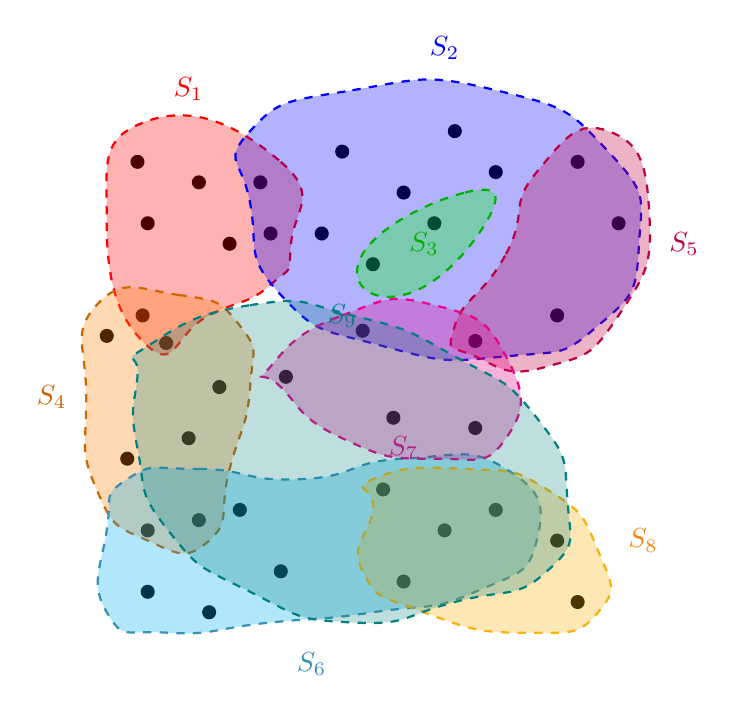
\begin{tikzpicture}[
    scale=1.3,
    node distance=1cm,
    element/.style={circle, draw, thick, fill=black, minimum size=0.15cm, inner sep=0pt},
    arrow/.style={->, thick}
]

% Universe elements - scattered randomly across the plane (35 elements with varied distribution)
\node[element] at (0.4, 3.9) {};
\node[element] at (0.9, 4.3) {};
\node[element] at (1.2, 3.7) {};
\node[element] at (0.35, 3) {};
\node[element] at (1.5, 4.3) {};
\node[element] at (0.3, 4.5) {};
\node[element] at (1.6, 3.8) {};  % SHARED by S1 and S2
\node[element] at (0.58, 2.73) {};  % SHARED by S1 and S4

\node[element] at (2.3, 4.6) {};
\node[element] at (2.9, 4.2) {};
\node[element] at (2.1, 3.8) {};
\node[element] at (3.4, 4.8) {};
\node[element] at (3.8, 4.4) {};
\node[element] at (2.6, 3.5) {};
\node[element] at (3.2, 3.9) {};

\node[element] at (4.6, 4.5) {};
\node[element] at (5, 3.9) {};
\node[element] at (4.4, 3) {};

\node[element] at (0, 2.8) {};
\node[element] at (1.1, 2.3) {};
\node[element] at (0.8, 1.8) {};
\node[element] at (0.2, 1.6) {};

\node[element] at (2.5, 2.85) {};
\node[element] at (3.6, 1.9) {};
\node[element] at (2.8, 2) {};
\node[element] at (3.6, 2.75) {};
\node[element] at (1.75, 2.4) {};

\node[element] at (0.9, 1.0) {};  % SHARED by S4 and S6
\node[element] at (0.4, 0.9) {};
\node[element] at (1.3, 1.1) {};
\node[element] at (0.4, 0.3) {};
\node[element] at (1.7, 0.5) {};
\node[element] at (1.0, 0.1) {};

\node[element] at (2.7, 1.3) {};
\node[element] at (3.3, 0.9) {};
\node[element] at (2.9, 0.4) {};
\node[element] at (3.8, 1.1) {};
\node[element] at (4.4, 0.8) {};
\node[element] at (4.6, 0.2) {};

% Set S1 (red) - includes (0.4,3.9) (0.9,4.3) (1.2,3.7) (0.6,3.2) (1.5,4.1) (0.3,4.5) + SHARED (1.6,4.0) (0.9,2.9)
\draw[thick, dashed, red, fill=red, fill opacity=0.3] 
    plot[smooth cycle, tension=1.0] coordinates {(0.4,4.9) (1.7,4.5) (1.8,3.7) (1.6,3.3) (1.0, 3) (0.4,2.7) (0.0,3.9)};
\node[above] at (0.8,5.0) {\textcolor{red}{$S_1$}};

% Set S2 (blue) - includes (2.3,4.6) (2.9,4.2) (2.1,3.8) (3.4,4.8) (3.8,4.4) (2.6,3.5) (3.2,3.9) (4.3,4.5) (4.7,3.9) (4.1,3.4) + SHARED (1.6,4.0)
\draw[thick, dashed, blue, fill=blue, fill opacity=0.3]
    plot[smooth cycle, tension=1.0] coordinates {(1.4,4.8) (2.4,5.2) (3.8,5.2) (4.9,4.6) (5.2,3.7) (4.8,2.9) (3.9,2.6) (2.7,2.7) (1.7,3.2) (1.4,4.1)};
\node[above] at (3.3,5.4) {\textcolor{blue}{$S_2$}};

% Set S3 (green) - small subset inside S2: (2.6,3.5) (3.2,3.9)
\draw[thick, dashed, green!70!black, fill=green, fill opacity=0.3]
    plot[smooth cycle, tension=1.0] coordinates {(2.5,3.6) (3.5,4.2) (3.7,3.9) (2.9,3.2)};
\node at (3.1,3.7) {\textcolor{green!70!black}{$S_3$}};

% Set S4 (orange) - includes (0.5,2.5) (1.1,2.8) (0.8,2.0) (0.2,1.6) + SHARED (0.9,1.0) (0.9,2.9)
\draw[thick, dashed, orange!80!black, fill=orange, fill opacity=0.3]
    plot[smooth cycle, tension=1.0] coordinates {(-0.1,3.1) (0.7,3.2) (1.3,2.9) (1.4,2.3) (1.2,1.5) (1.0,0.8) (0.4,0.8) (-0.1,1.3) (-0.2,2.2)};
\node[left] at (-0.3,2.2) {\textcolor{orange!80!black}{$S_4$}};

% Set S5 (purple) - right side elongated: (3.6,2.6) overlaps with S2 for (4.3,4.5) (4.7,3.9) (4.1,3.4)
\draw[thick, dashed, purple, fill=purple, fill opacity=0.3]
    plot[smooth cycle, tension=1.0] coordinates {(3.4,2.9) (3.9,3.6) (4.2,4.4) (4.9,4.8) (5.3,4.0) (5.0,3.0) (4.3,2.5) (3.6,2.6)};
\node[right] at (5.4,3.7) {\textcolor{purple}{$S_5$}};

% Set S6 (cyan) - includes (0.9,1.0) (0.7,0.8) (1.3,1.1) (0.4,0.3) (1.7,0.5) (1.0,0.1) (2.7,1.3) (3.3,0.9) (2.9,0.4) (3.8,1.1)
\draw[thick, dashed, cyan!70!black, fill=cyan, fill opacity=0.3]
    plot[smooth cycle, tension=1.0] coordinates {(0.2,1.4) (0.9,1.5) (1.9,1.4) (2.9,1.6) (3.9,1.5) (4.2,0.8) (3.6,0.3) (2.6,0.1) (1.6,0.0) (0.6,-0.1) (0.0,0.1) (0.0,0.9)};
\node[below] at (2.0,-0.2) {\textcolor{cyan!70!black}{$S_6$}};

% Set S7 (magenta) - includes (2.5,2.9) (3.1,2.4) (2.8,1.9) (1.9,2.2)
\draw[thick, dashed, magenta, fill=magenta, fill opacity=0.3]
    plot[smooth cycle, tension=1.0] coordinates {(1.6,2.5) (2.3,3.0) (3.2,3.1) (3.9,2.6) (3.9,1.8) (3.2,1.6) (2.3,1.8) (1.7,2.3)};
\node[above] at (2.9,1.5) {\textcolor{magenta}{$S_7$}};

% Set S8 (yellow!70!red) - includes (3.8,1.1) (4.4,0.6) (3.3,0.9) (2.9,0.4)
\draw[thick, dashed, yellow!70!red, fill=yellow!70!red, fill opacity=0.3]
    plot[smooth cycle, tension=1.0] coordinates {(2.6,1.4) (3.5,1.5) (4.3,1.3) (4.8,0.7) (4.8,0.1) (4.1,-0.1) (3.1,0.1) (2.5,0.5) (2.6,1.1)};
\node[right] at (5.0,0.8) {\textcolor{yellow!50!red}{$S_8$}};

% Set S9 (teal) - large blob filling gaps: overlaps with others to ensure complete coverage
\draw[thick, dashed, teal, fill=teal, fill opacity=0.25]
    plot[smooth cycle, tension=1.0] coordinates {(0.4,2.7) (1.4,3.1) (2.4,3.0) (3.4,2.6) (4.2,2.0) (4.5,1.2) (4.3,0.5) (3.4,0.2) (2.4,0.0) (1.4,0.3) (0.6,0.9) (0.3,1.7) (0.3,2.4)};
\node[below] at (2.3,3.2) {\textcolor{teal}{$S_9$}};

\end{tikzpicture}
}
\normalsize
\caption*{(a) Universe and sets}
\end{minipage}
\hfill
\begin{minipage}[t]{0.35\textwidth}
\centering
\scalebox{0.57}{
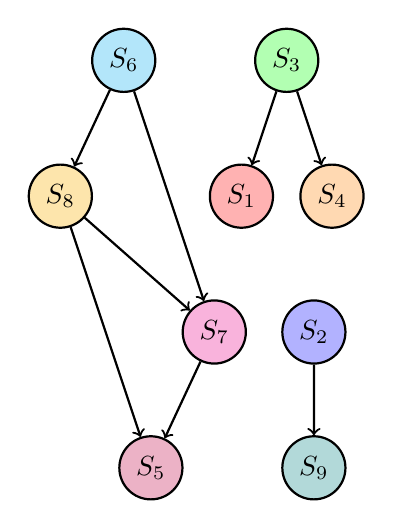
\begin{tikzpicture}[
    scale=1.15,
    node distance=1cm,
    set/.style={circle, draw, thick, minimum size=0.65cm},
    arrow/.style={->, thick}
]

% Precedence DAG with specified precedence constraints

% Component with S6 (left, wider)
\node[set, fill=cyan!30] (s6) at (0,0) {$S_6$};
\node[set, fill=yellow!70!red!30] (s8) at (-0.7,-1.5) {$S_8$};
\node[set, fill=magenta!30] (s7) at (1,-3) {$S_7$};
\node[set, fill=purple!30] (s5) at (0.3,-4.5) {$S_5$};

% Component with S3 (right top)
\node[set, fill=green!30] (s3) at (1.8,0) {$S_3$};
\node[set, fill=red!30] (s1) at (1.3,-1.5) {$S_1$};
\node[set, fill=orange!30] (s4) at (2.3,-1.5) {$S_4$};

% Component with S2 (right bottom)
\node[set, fill=blue!30] (s2) at (2.1,-3) {$S_2$};
\node[set, fill=teal!30] (s9) at (2.1,-4.5) {$S_9$};

% Precedence constraints (all arrows go down)
\draw[arrow] (s3) -- (s1);
\draw[arrow] (s3) -- (s4);
\draw[arrow] (s6) -- (s7);
\draw[arrow] (s6) -- (s8);
\draw[arrow] (s8) -- (s7);
\draw[arrow] (s8) -- (s5);
\draw[arrow] (s7) -- (s5);
\draw[arrow] (s2) -- (s9);

\end{tikzpicture}
}
\normalsize
\caption*{(b) Precedence}
\end{minipage}

\vspace{0.5cm}

\begin{minipage}[t]{\textwidth}
\centering
\scalebox{0.765}{
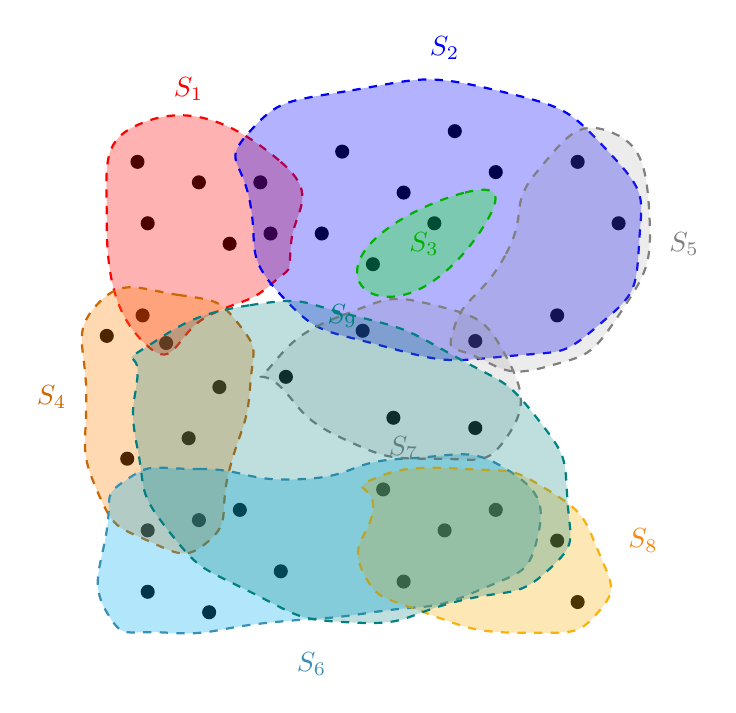
\begin{tikzpicture}[
    scale=1.3,
    node distance=1cm,
    element/.style={circle, draw, thick, fill=black, minimum size=0.15cm, inner sep=0pt},
    arrow/.style={->, thick}
]

% Universe elements - scattered randomly across the plane (35 elements with varied distribution)
\node[element] at (0.4, 3.9) {};
\node[element] at (0.9, 4.3) {};
\node[element] at (1.2, 3.7) {};
\node[element] at (0.35, 3) {};
\node[element] at (1.5, 4.3) {};
\node[element] at (0.3, 4.5) {};
\node[element] at (1.6, 3.8) {};  % SHARED by S1 and S2
\node[element] at (0.58, 2.73) {};  % SHARED by S1 and S4

\node[element] at (2.3, 4.6) {};
\node[element] at (2.9, 4.2) {};
\node[element] at (2.1, 3.8) {};
\node[element] at (3.4, 4.8) {};
\node[element] at (3.8, 4.4) {};
\node[element] at (2.6, 3.5) {};
\node[element] at (3.2, 3.9) {};

\node[element] at (4.6, 4.5) {};
\node[element] at (5, 3.9) {};
\node[element] at (4.4, 3) {};

\node[element] at (0, 2.8) {};
\node[element] at (1.1, 2.3) {};
\node[element] at (0.8, 1.8) {};
\node[element] at (0.2, 1.6) {};

\node[element] at (2.5, 2.85) {};
\node[element] at (3.6, 1.9) {};
\node[element] at (2.8, 2) {};
\node[element] at (3.6, 2.75) {};
\node[element] at (1.75, 2.4) {};

\node[element] at (0.9, 1.0) {};  % SHARED by S4 and S6
\node[element] at (0.4, 0.9) {};
\node[element] at (1.3, 1.1) {};
\node[element] at (0.4, 0.3) {};
\node[element] at (1.7, 0.5) {};
\node[element] at (1.0, 0.1) {};

\node[element] at (2.7, 1.3) {};
\node[element] at (3.3, 0.9) {};
\node[element] at (2.9, 0.4) {};
\node[element] at (3.8, 1.1) {};
\node[element] at (4.4, 0.8) {};
\node[element] at (4.6, 0.2) {};

% Set S1 (red) - SELECTED
\draw[thick, dashed, red, fill=red, fill opacity=0.3] 
    plot[smooth cycle, tension=1.0] coordinates {(0.4,4.9) (1.7,4.5) (1.8,3.7) (1.6,3.3) (1.0, 3) (0.4,2.7) (0.0,3.9)};
\node[above] at (0.8,5.0) {\textcolor{red}{\textbf{$S_1$}}};

% Set S2 (blue) - SELECTED
\draw[thick, dashed, blue, fill=blue, fill opacity=0.3]
    plot[smooth cycle, tension=1.0] coordinates {(1.4,4.8) (2.4,5.2) (3.8,5.2) (4.9,4.6) (5.2,3.7) (4.8,2.9) (3.9,2.6) (2.7,2.7) (1.7,3.2) (1.4,4.1)};
\node[above] at (3.3,5.4) {\textcolor{blue}{\textbf{$S_2$}}};

% Set S3 (green) - SELECTED
\draw[thick, dashed, green!70!black, fill=green, fill opacity=0.3]
    plot[smooth cycle, tension=1.0] coordinates {(2.5,3.6) (3.5,4.2) (3.7,3.9) (2.9,3.2)};
\node at (3.1,3.7) {\textcolor{green!70!black}{\textbf{$S_3$}}};

% Set S4 (orange) - SELECTED
\draw[thick, dashed, orange!80!black, fill=orange, fill opacity=0.3]
    plot[smooth cycle, tension=1.0] coordinates {(-0.1,3.1) (0.7,3.2) (1.3,2.9) (1.4,2.3) (1.2,1.5) (1.0,0.8) (0.4,0.8) (-0.1,1.3) (-0.2,2.2)};
\node[left] at (-0.3,2.2) {\textcolor{orange!80!black}{\textbf{$S_4$}}};

% Set S5 (purple) - NOT SELECTED (grayed out)
\draw[thick, dashed, gray, fill=gray, fill opacity=0.15]
    plot[smooth cycle, tension=1.0] coordinates {(3.4,2.9) (3.9,3.6) (4.2,4.4) (4.9,4.8) (5.3,4.0) (5.0,3.0) (4.3,2.5) (3.6,2.6)};
\node[right] at (5.4,3.7) {\textcolor{gray}{$S_5$}};

% Set S6 (cyan) - SELECTED
\draw[thick, dashed, cyan!70!black, fill=cyan, fill opacity=0.3]
    plot[smooth cycle, tension=1.0] coordinates {(0.2,1.4) (0.9,1.5) (1.9,1.4) (2.9,1.6) (3.9,1.5) (4.2,0.8) (3.6,0.3) (2.6,0.1) (1.6,0.0) (0.6,-0.1) (0.0,0.1) (0.0,0.9)};
\node[below] at (2.0,-0.2) {\textcolor{cyan!70!black}{\textbf{$S_6$}}};

% Set S7 (magenta) - NOT SELECTED (grayed out)
\draw[thick, dashed, gray, fill=gray, fill opacity=0.15]
    plot[smooth cycle, tension=1.0] coordinates {(1.6,2.5) (2.3,3.0) (3.2,3.1) (3.9,2.6) (3.9,1.8) (3.2,1.6) (2.3,1.8) (1.7,2.3)};
\node[above] at (2.9,1.5) {\textcolor{gray}{$S_7$}};

% Set S8 (yellow!70!red) - SELECTED
\draw[thick, dashed, yellow!70!red, fill=yellow!70!red, fill opacity=0.3]
    plot[smooth cycle, tension=1.0] coordinates {(2.6,1.4) (3.5,1.5) (4.3,1.3) (4.8,0.7) (4.8,0.1) (4.1,-0.1) (3.1,0.1) (2.5,0.5) (2.6,1.1)};
\node[right] at (5.0,0.8) {\textcolor{yellow!50!red}{\textbf{$S_8$}}};

% Set S9 (teal) - SELECTED
\draw[thick, dashed, teal, fill=teal, fill opacity=0.25]
    plot[smooth cycle, tension=1.0] coordinates {(0.4,2.7) (1.4,3.1) (2.4,3.0) (3.4,2.6) (4.2,2.0) (4.5,1.2) (4.3,0.5) (3.4,0.2) (2.4,0.0) (1.4,0.3) (0.6,0.9) (0.3,1.7) (0.3,2.4)};
\node[below] at (2.3,3.2) {\textcolor{teal}{\textbf{$S_9$}}};

\end{tikzpicture}
}
\normalsize
\caption*{(c) Solution: $\{S_1, S_2, S_6, S_8, S_9\}$ (in color)}
\end{minipage}


% \caption{Example of a PCCP instance with 39 elements and 9 covering sets. (a) Universe with covering sets. (b) Precedence DAG with three components. (c) Solution using 7 selected sets (colored).}\label{fig:pccp_example}
% \end{figure}

% \begin{figure}[h]
% \centering
% \centering

\begin{minipage}[t]{0.6\textwidth}
\centering
\scalebox{0.57}{
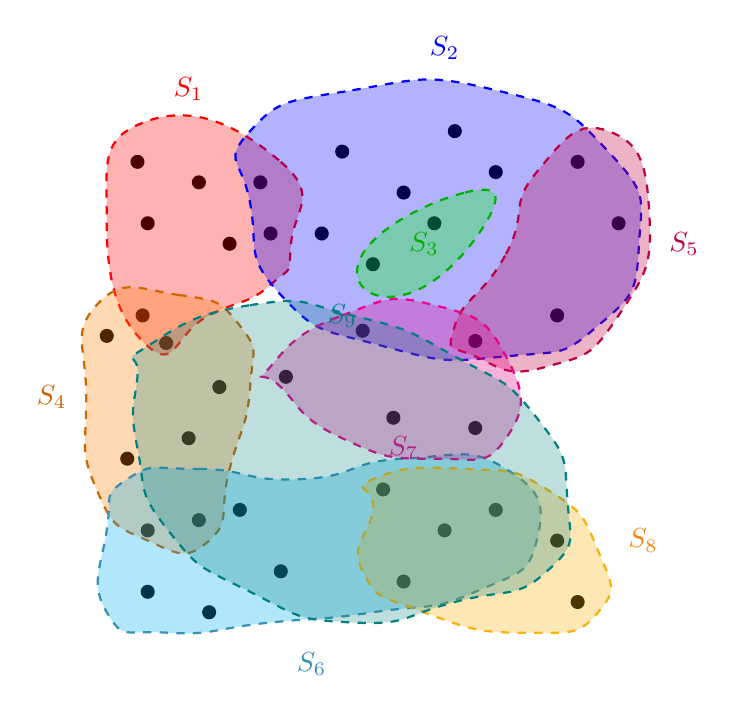
\begin{tikzpicture}[
    scale=1.3,
    node distance=1cm,
    element/.style={circle, draw, thick, fill=black, minimum size=0.15cm, inner sep=0pt},
    arrow/.style={->, thick}
]

% Universe elements - scattered randomly across the plane (35 elements with varied distribution)
\node[element] at (0.4, 3.9) {};
\node[element] at (0.9, 4.3) {};
\node[element] at (1.2, 3.7) {};
\node[element] at (0.35, 3) {};
\node[element] at (1.5, 4.3) {};
\node[element] at (0.3, 4.5) {};
\node[element] at (1.6, 3.8) {};  % SHARED by S1 and S2
\node[element] at (0.58, 2.73) {};  % SHARED by S1 and S4

\node[element] at (2.3, 4.6) {};
\node[element] at (2.9, 4.2) {};
\node[element] at (2.1, 3.8) {};
\node[element] at (3.4, 4.8) {};
\node[element] at (3.8, 4.4) {};
\node[element] at (2.6, 3.5) {};
\node[element] at (3.2, 3.9) {};

\node[element] at (4.6, 4.5) {};
\node[element] at (5, 3.9) {};
\node[element] at (4.4, 3) {};

\node[element] at (0, 2.8) {};
\node[element] at (1.1, 2.3) {};
\node[element] at (0.8, 1.8) {};
\node[element] at (0.2, 1.6) {};

\node[element] at (2.5, 2.85) {};
\node[element] at (3.6, 1.9) {};
\node[element] at (2.8, 2) {};
\node[element] at (3.6, 2.75) {};
\node[element] at (1.75, 2.4) {};

\node[element] at (0.9, 1.0) {};  % SHARED by S4 and S6
\node[element] at (0.4, 0.9) {};
\node[element] at (1.3, 1.1) {};
\node[element] at (0.4, 0.3) {};
\node[element] at (1.7, 0.5) {};
\node[element] at (1.0, 0.1) {};

\node[element] at (2.7, 1.3) {};
\node[element] at (3.3, 0.9) {};
\node[element] at (2.9, 0.4) {};
\node[element] at (3.8, 1.1) {};
\node[element] at (4.4, 0.8) {};
\node[element] at (4.6, 0.2) {};

% Set S1 (red) - includes (0.4,3.9) (0.9,4.3) (1.2,3.7) (0.6,3.2) (1.5,4.1) (0.3,4.5) + SHARED (1.6,4.0) (0.9,2.9)
\draw[thick, dashed, red, fill=red, fill opacity=0.3] 
    plot[smooth cycle, tension=1.0] coordinates {(0.4,4.9) (1.7,4.5) (1.8,3.7) (1.6,3.3) (1.0, 3) (0.4,2.7) (0.0,3.9)};
\node[above] at (0.8,5.0) {\textcolor{red}{$S_1$}};

% Set S2 (blue) - includes (2.3,4.6) (2.9,4.2) (2.1,3.8) (3.4,4.8) (3.8,4.4) (2.6,3.5) (3.2,3.9) (4.3,4.5) (4.7,3.9) (4.1,3.4) + SHARED (1.6,4.0)
\draw[thick, dashed, blue, fill=blue, fill opacity=0.3]
    plot[smooth cycle, tension=1.0] coordinates {(1.4,4.8) (2.4,5.2) (3.8,5.2) (4.9,4.6) (5.2,3.7) (4.8,2.9) (3.9,2.6) (2.7,2.7) (1.7,3.2) (1.4,4.1)};
\node[above] at (3.3,5.4) {\textcolor{blue}{$S_2$}};

% Set S3 (green) - small subset inside S2: (2.6,3.5) (3.2,3.9)
\draw[thick, dashed, green!70!black, fill=green, fill opacity=0.3]
    plot[smooth cycle, tension=1.0] coordinates {(2.5,3.6) (3.5,4.2) (3.7,3.9) (2.9,3.2)};
\node at (3.1,3.7) {\textcolor{green!70!black}{$S_3$}};

% Set S4 (orange) - includes (0.5,2.5) (1.1,2.8) (0.8,2.0) (0.2,1.6) + SHARED (0.9,1.0) (0.9,2.9)
\draw[thick, dashed, orange!80!black, fill=orange, fill opacity=0.3]
    plot[smooth cycle, tension=1.0] coordinates {(-0.1,3.1) (0.7,3.2) (1.3,2.9) (1.4,2.3) (1.2,1.5) (1.0,0.8) (0.4,0.8) (-0.1,1.3) (-0.2,2.2)};
\node[left] at (-0.3,2.2) {\textcolor{orange!80!black}{$S_4$}};

% Set S5 (purple) - right side elongated: (3.6,2.6) overlaps with S2 for (4.3,4.5) (4.7,3.9) (4.1,3.4)
\draw[thick, dashed, purple, fill=purple, fill opacity=0.3]
    plot[smooth cycle, tension=1.0] coordinates {(3.4,2.9) (3.9,3.6) (4.2,4.4) (4.9,4.8) (5.3,4.0) (5.0,3.0) (4.3,2.5) (3.6,2.6)};
\node[right] at (5.4,3.7) {\textcolor{purple}{$S_5$}};

% Set S6 (cyan) - includes (0.9,1.0) (0.7,0.8) (1.3,1.1) (0.4,0.3) (1.7,0.5) (1.0,0.1) (2.7,1.3) (3.3,0.9) (2.9,0.4) (3.8,1.1)
\draw[thick, dashed, cyan!70!black, fill=cyan, fill opacity=0.3]
    plot[smooth cycle, tension=1.0] coordinates {(0.2,1.4) (0.9,1.5) (1.9,1.4) (2.9,1.6) (3.9,1.5) (4.2,0.8) (3.6,0.3) (2.6,0.1) (1.6,0.0) (0.6,-0.1) (0.0,0.1) (0.0,0.9)};
\node[below] at (2.0,-0.2) {\textcolor{cyan!70!black}{$S_6$}};

% Set S7 (magenta) - includes (2.5,2.9) (3.1,2.4) (2.8,1.9) (1.9,2.2)
\draw[thick, dashed, magenta, fill=magenta, fill opacity=0.3]
    plot[smooth cycle, tension=1.0] coordinates {(1.6,2.5) (2.3,3.0) (3.2,3.1) (3.9,2.6) (3.9,1.8) (3.2,1.6) (2.3,1.8) (1.7,2.3)};
\node[above] at (2.9,1.5) {\textcolor{magenta}{$S_7$}};

% Set S8 (yellow!70!red) - includes (3.8,1.1) (4.4,0.6) (3.3,0.9) (2.9,0.4)
\draw[thick, dashed, yellow!70!red, fill=yellow!70!red, fill opacity=0.3]
    plot[smooth cycle, tension=1.0] coordinates {(2.6,1.4) (3.5,1.5) (4.3,1.3) (4.8,0.7) (4.8,0.1) (4.1,-0.1) (3.1,0.1) (2.5,0.5) (2.6,1.1)};
\node[right] at (5.0,0.8) {\textcolor{yellow!50!red}{$S_8$}};

% Set S9 (teal) - large blob filling gaps: overlaps with others to ensure complete coverage
\draw[thick, dashed, teal, fill=teal, fill opacity=0.25]
    plot[smooth cycle, tension=1.0] coordinates {(0.4,2.7) (1.4,3.1) (2.4,3.0) (3.4,2.6) (4.2,2.0) (4.5,1.2) (4.3,0.5) (3.4,0.2) (2.4,0.0) (1.4,0.3) (0.6,0.9) (0.3,1.7) (0.3,2.4)};
\node[below] at (2.3,3.2) {\textcolor{teal}{$S_9$}};

\end{tikzpicture}
}
\normalsize
\caption*{(a) Universe and sets}
\end{minipage}
\hfill
\begin{minipage}[t]{0.35\textwidth}
\centering
\scalebox{0.57}{
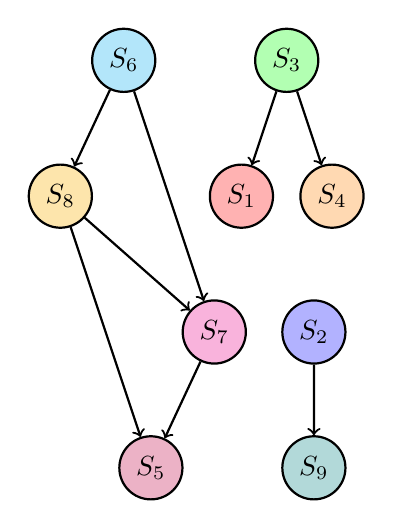
\begin{tikzpicture}[
    scale=1.15,
    node distance=1cm,
    set/.style={circle, draw, thick, minimum size=0.65cm},
    arrow/.style={->, thick}
]

% Precedence DAG with specified precedence constraints

% Component with S6 (left, wider)
\node[set, fill=cyan!30] (s6) at (0,0) {$S_6$};
\node[set, fill=yellow!70!red!30] (s8) at (-0.7,-1.5) {$S_8$};
\node[set, fill=magenta!30] (s7) at (1,-3) {$S_7$};
\node[set, fill=purple!30] (s5) at (0.3,-4.5) {$S_5$};

% Component with S3 (right top)
\node[set, fill=green!30] (s3) at (1.8,0) {$S_3$};
\node[set, fill=red!30] (s1) at (1.3,-1.5) {$S_1$};
\node[set, fill=orange!30] (s4) at (2.3,-1.5) {$S_4$};

% Component with S2 (right bottom)
\node[set, fill=blue!30] (s2) at (2.1,-3) {$S_2$};
\node[set, fill=teal!30] (s9) at (2.1,-4.5) {$S_9$};

% Precedence constraints (all arrows go down)
\draw[arrow] (s3) -- (s1);
\draw[arrow] (s3) -- (s4);
\draw[arrow] (s6) -- (s7);
\draw[arrow] (s6) -- (s8);
\draw[arrow] (s8) -- (s7);
\draw[arrow] (s8) -- (s5);
\draw[arrow] (s7) -- (s5);
\draw[arrow] (s2) -- (s9);

\end{tikzpicture}
}
\normalsize
\caption*{(b) Precedence}
\end{minipage}

\vspace{0.5cm}

\begin{minipage}[t]{\textwidth}
\centering
\scalebox{0.765}{
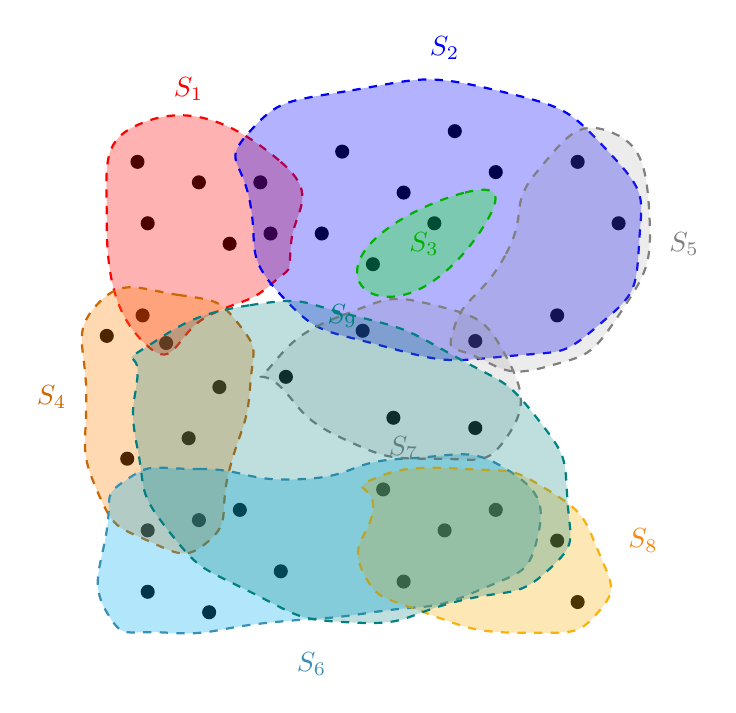
\begin{tikzpicture}[
    scale=1.3,
    node distance=1cm,
    element/.style={circle, draw, thick, fill=black, minimum size=0.15cm, inner sep=0pt},
    arrow/.style={->, thick}
]

% Universe elements - scattered randomly across the plane (35 elements with varied distribution)
\node[element] at (0.4, 3.9) {};
\node[element] at (0.9, 4.3) {};
\node[element] at (1.2, 3.7) {};
\node[element] at (0.35, 3) {};
\node[element] at (1.5, 4.3) {};
\node[element] at (0.3, 4.5) {};
\node[element] at (1.6, 3.8) {};  % SHARED by S1 and S2
\node[element] at (0.58, 2.73) {};  % SHARED by S1 and S4

\node[element] at (2.3, 4.6) {};
\node[element] at (2.9, 4.2) {};
\node[element] at (2.1, 3.8) {};
\node[element] at (3.4, 4.8) {};
\node[element] at (3.8, 4.4) {};
\node[element] at (2.6, 3.5) {};
\node[element] at (3.2, 3.9) {};

\node[element] at (4.6, 4.5) {};
\node[element] at (5, 3.9) {};
\node[element] at (4.4, 3) {};

\node[element] at (0, 2.8) {};
\node[element] at (1.1, 2.3) {};
\node[element] at (0.8, 1.8) {};
\node[element] at (0.2, 1.6) {};

\node[element] at (2.5, 2.85) {};
\node[element] at (3.6, 1.9) {};
\node[element] at (2.8, 2) {};
\node[element] at (3.6, 2.75) {};
\node[element] at (1.75, 2.4) {};

\node[element] at (0.9, 1.0) {};  % SHARED by S4 and S6
\node[element] at (0.4, 0.9) {};
\node[element] at (1.3, 1.1) {};
\node[element] at (0.4, 0.3) {};
\node[element] at (1.7, 0.5) {};
\node[element] at (1.0, 0.1) {};

\node[element] at (2.7, 1.3) {};
\node[element] at (3.3, 0.9) {};
\node[element] at (2.9, 0.4) {};
\node[element] at (3.8, 1.1) {};
\node[element] at (4.4, 0.8) {};
\node[element] at (4.6, 0.2) {};

% Set S1 (red) - SELECTED
\draw[thick, dashed, red, fill=red, fill opacity=0.3] 
    plot[smooth cycle, tension=1.0] coordinates {(0.4,4.9) (1.7,4.5) (1.8,3.7) (1.6,3.3) (1.0, 3) (0.4,2.7) (0.0,3.9)};
\node[above] at (0.8,5.0) {\textcolor{red}{\textbf{$S_1$}}};

% Set S2 (blue) - SELECTED
\draw[thick, dashed, blue, fill=blue, fill opacity=0.3]
    plot[smooth cycle, tension=1.0] coordinates {(1.4,4.8) (2.4,5.2) (3.8,5.2) (4.9,4.6) (5.2,3.7) (4.8,2.9) (3.9,2.6) (2.7,2.7) (1.7,3.2) (1.4,4.1)};
\node[above] at (3.3,5.4) {\textcolor{blue}{\textbf{$S_2$}}};

% Set S3 (green) - SELECTED
\draw[thick, dashed, green!70!black, fill=green, fill opacity=0.3]
    plot[smooth cycle, tension=1.0] coordinates {(2.5,3.6) (3.5,4.2) (3.7,3.9) (2.9,3.2)};
\node at (3.1,3.7) {\textcolor{green!70!black}{\textbf{$S_3$}}};

% Set S4 (orange) - SELECTED
\draw[thick, dashed, orange!80!black, fill=orange, fill opacity=0.3]
    plot[smooth cycle, tension=1.0] coordinates {(-0.1,3.1) (0.7,3.2) (1.3,2.9) (1.4,2.3) (1.2,1.5) (1.0,0.8) (0.4,0.8) (-0.1,1.3) (-0.2,2.2)};
\node[left] at (-0.3,2.2) {\textcolor{orange!80!black}{\textbf{$S_4$}}};

% Set S5 (purple) - NOT SELECTED (grayed out)
\draw[thick, dashed, gray, fill=gray, fill opacity=0.15]
    plot[smooth cycle, tension=1.0] coordinates {(3.4,2.9) (3.9,3.6) (4.2,4.4) (4.9,4.8) (5.3,4.0) (5.0,3.0) (4.3,2.5) (3.6,2.6)};
\node[right] at (5.4,3.7) {\textcolor{gray}{$S_5$}};

% Set S6 (cyan) - SELECTED
\draw[thick, dashed, cyan!70!black, fill=cyan, fill opacity=0.3]
    plot[smooth cycle, tension=1.0] coordinates {(0.2,1.4) (0.9,1.5) (1.9,1.4) (2.9,1.6) (3.9,1.5) (4.2,0.8) (3.6,0.3) (2.6,0.1) (1.6,0.0) (0.6,-0.1) (0.0,0.1) (0.0,0.9)};
\node[below] at (2.0,-0.2) {\textcolor{cyan!70!black}{\textbf{$S_6$}}};

% Set S7 (magenta) - NOT SELECTED (grayed out)
\draw[thick, dashed, gray, fill=gray, fill opacity=0.15]
    plot[smooth cycle, tension=1.0] coordinates {(1.6,2.5) (2.3,3.0) (3.2,3.1) (3.9,2.6) (3.9,1.8) (3.2,1.6) (2.3,1.8) (1.7,2.3)};
\node[above] at (2.9,1.5) {\textcolor{gray}{$S_7$}};

% Set S8 (yellow!70!red) - SELECTED
\draw[thick, dashed, yellow!70!red, fill=yellow!70!red, fill opacity=0.3]
    plot[smooth cycle, tension=1.0] coordinates {(2.6,1.4) (3.5,1.5) (4.3,1.3) (4.8,0.7) (4.8,0.1) (4.1,-0.1) (3.1,0.1) (2.5,0.5) (2.6,1.1)};
\node[right] at (5.0,0.8) {\textcolor{yellow!50!red}{\textbf{$S_8$}}};

% Set S9 (teal) - SELECTED
\draw[thick, dashed, teal, fill=teal, fill opacity=0.25]
    plot[smooth cycle, tension=1.0] coordinates {(0.4,2.7) (1.4,3.1) (2.4,3.0) (3.4,2.6) (4.2,2.0) (4.5,1.2) (4.3,0.5) (3.4,0.2) (2.4,0.0) (1.4,0.3) (0.6,0.9) (0.3,1.7) (0.3,2.4)};
\node[below] at (2.3,3.2) {\textcolor{teal}{\textbf{$S_9$}}};

\end{tikzpicture}
}
\normalsize
\caption*{(c) Solution: $\{S_1, S_2, S_6, S_8, S_9\}$ (in color)}
\end{minipage}


% \caption{Example of a PCCP instance with 39 elements and 9 covering sets. (a) Universe with covering sets. (b) Precedence DAG with three components. (c) Solution using 7 selected sets (colored).}\label{fig:pccp_example}
% \end{figure}

Table~\ref{tab:results} summarizes all results, also including best known from literature.
\begin{table}[htb]
\caption{Approximation guarantees for covering and decision tree problems under different precedence constraints. (* denotes new results, ** denotes previously unmentioned corollaries of known results).}
\label{tab:results}
\centering
{
\small
\begin{tabular}{lC{0.14\linewidth}C{0.14\linewidth}C{0.14\linewidth}C{0.14\linewidth}C{0.14\linewidth}}
\toprule
\textbf{precedence} & \textbf{$\ProblemPCSC$} & \textbf{$\ProblemBPCSC$} & \textbf{$\ProblemPCMSSC$} & \textbf{$\ProblemPCWCDT$} & \textbf{$\ProblemPCACDT$} \\
\midrule
none & $\cO(\log n)$ \cite{ThresholdLnNSetCover} & $\br{1, \frac{e}{e-1}}$ \cite{TheBudgetedMaximumCoverageProblem} & $4$ \cite{ApproximatingMinSumSetCover} & $\cO(\log n)$** & $\cO(\log n)$ \cite{ApproximatingDecisionTreesMultiwayBranches} \\
\midrule
inforest & $\br{1, \frac{e}{e-1}}$ (Thm.~\ref{thm:BPCSC-inforest}) & $\br{1, \frac{e}{e-1}}$ (Thm.~\ref{thm:BPCSC-inforest}) & $\cO(1)$* & $\cO(\log n)$* & $\cO(\log(m\!+\!n))$* \\
\midrule
outforest & $\br{\cO(\log n), 4}$ (Thm.~\ref{thm:BPCSC-outforest}) & $\br{\cO(\log n), 4}$ (Thm.~\ref{thm:BPCSC-outforest}) & $\br{\cO(\log n), 4}$* & $\cO(\log^2 n)$* & $\cO(\log^2(m\!+\!n))$* \\
\midrule
general & $\cO(\sqrt{m}f)$ (Thm.~\ref{thm:generalPCSC}) & $\br{\sqrt{m\cdot H_n}\!+\!1, 1}$ (Thm.~\ref{thm:BPCSC}) & $\cO(\sqrt{m})$ (Thm.~\ref{thm:generalPCMSSC}) & $\cO(\sqrt{m}\log n)$ (Thm.~\ref{thm:generalPCWCDT}) & $\cO(\sqrt{m}\log^{3/2}(m\!+\!n))$ (Thm.~\ref{thm:generalPCACDT}) \\
\bottomrule
\end{tabular}
}
\end{table}

\begin{figure}[h]
\centering
\begin{tikzpicture}[
    node distance=2.5cm and 3cm,
    problem/.style={rectangle, draw, very thick, minimum width=2.2cm, minimum height=1cm, align=center, font=\small},
    arrow/.style={->, very thick}
]

% Third row (define first for positioning)
\node[problem] (pcmssc) {PCMSSC};
\node[problem, right=3cm of pcmssc] (pcsc) {PCSC};

% Second row (above pcsc)
\node[problem, above right=0.7cm and 2cm of pcsc] (gst) {GST};

% Top row (above gst)
\node[problem, above left=0.6cm and 1.5cm of gst] (mdpcs) {MDPCS};

% Bottom row
\node[problem, below=0.6cm of pcmssc] (pcacal) {PCACAL};
\node[problem, below=0.6cm of pcsc] (pcwcal) {PCWCAL};
\node[problem, right=3cm of pcwcal] (pctc) {PCTC};

% Arrows
\draw[arrow] (mdpcs) -- (gst);
\draw[arrow] (mdpcs) -- (pcsc);
\draw[arrow] (mdpcs) -- (pcmssc);
\draw[arrow] (gst) -- (pcsc);
\draw[arrow] (pcsc) -- (pctc);
\draw[arrow] (pcsc) -- (pcwcal);
\draw[arrow] (pcmssc) -- (pcacal);

\end{tikzpicture}

\caption{Relationships between covering and decision tree problems, $\Pi_1 \to \Pi_2$ denotes that an approximation algorithm for problem $\Pi_1$ implies an approximation algorithm for problem $\Pi_2$.}\label{fig:reductions}
\end{figure}

\begin{figure}[h]
    \centering
    \begin{tikzpicture}[
    node distance=1.1cm and 2cm,
    problem/.style={rectangle, draw, very thick, minimum width=1.8cm, minimum height=0.8cm, align=center, font=\scriptsize},
    arrow/.style={->, very thick}
]

% Define positions based on the hand-drawn diagram
% Top level
\node[problem] (gst) at (-2, 0) {$\ProblemGST$};
\node[problem] (pds) at (2, 0) {$\ProblemPDS$};

% Middle level
\node[problem, below left=1.1cm and 0.5cm of pds] (fpcsc) {$\ProblemPCSC$};
\node[problem, below right=1.1cm and 0.5cm of pds] (fpcmssc) {$\ProblemPCMSSC$};

% Bottom level
\node[problem, below=1.1cm of fpcsc] (pcwcdt) {$\ProblemPCWCDT$};
\node[problem, below=1.1cm of fpcmssc] (pcacdt) {$\ProblemPCACDT$};

% Arrows with hyperlinks to sections
\draw[arrow] (gst) -- (fpcsc);
\draw[arrow] (pds) -- (fpcsc);
\draw[arrow] (pds) -- (fpcmssc);
\draw[arrow] (fpcsc) -- (pcwcdt);
\draw[arrow] (fpcsc) -- (pcacdt);
\draw[arrow] (fpcmssc) -- (pcacdt);

\end{tikzpicture}

    \caption{Inapproximability relations between problems, $\Pi_1 \to \Pi_2$ denotes that an inapproximability result for problem $\Pi_1$ implies an inapproximability result for problem $\Pi_2$.}
    \label{fig:hardness_diagram}
\end{figure}

\DD{tutaj bylby jakis wywod i intuicje jakie techniki sa nowe, generalnie trzebaby sie pochwalic pomyslami roznymi}

\subsection{Organization}